%----------------------------------------------------------------------------------------
%	PACKAGES AND OTHER DOCUMENT CONFIGURATIONS
%----------------------------------------------------------------------------------------

\documentclass[
	10pt, % Set the default font size, options include: 8pt, 9pt, 10pt, 11pt, 12pt, 14pt, 17pt, 20pt
	%t, % Uncomment to vertically align all slide content to the top of the slide, rather than the default centered
	%aspectratio=169, % Uncomment to set the aspect ratio to a 16:9 ratio which matches the aspect ratio of 1080p and 4K screens and projectors
	hmargin=1cm,vmargin=0cm,head=0.5cm,headsep=0pt,foot=0.5cm,margin=2cm
]{beamer}

% Hide navigation symbols
\setbeamertemplate{navigation symbols}{}
 
\usepackage{caption}
\captionsetup{labelformat=empty,labelsep=none}
\graphicspath{{images/}{./}} % Specifies where to look for included images (trailing slash required)
\usepackage{minted}
% \usepackage{setspace}
\linespread{1}
\usepackage{amsmath}
\usepackage{multirow}
\usepackage{color, colortbl}
\usepackage{xcolor}
\usepackage{booktabs} % Allows the use of \toprule, \midrule and \bottomrule for better rules in tables
\usepackage{graphicx}
\usepackage{minibox}
\renewcommand{\arraystretch}{1.2} % Default value: 1
\definecolor{darkGreen}{RGB}{9,150,3} 
\usepackage{tikz}

\newcommand{\tikzunderarrow}[2][black]{\tikz[baseline={(N.base)}]{
  \node[inner sep=0, outer sep=0](N) {#2};
  \draw[overlay, -latex, line width=.04em, #1]
    ([yshift=-.14em]N.south west) -- ([yshift=-.14em]N.south east);}}
\usepackage{ragged2e}
\tolerance=1
\emergencystretch=\maxdimen
\hyphenpenalty=10000
\hbadness=10000

%	SELECT LAYOUT THEME
%----------------------------------------------------------------------------------------
%
% Beamer comes with a number of default layout themes which change the colors and layouts of slides. Below is a list of all themes available, uncomment each in turn to see what they look like.

%\usetheme{default}
%\usetheme{AnnArbor}
%\usetheme{Antibes}
%\usetheme{Bergen}
%\usetheme{Berkeley}
% \usetheme{Berlin}
%\usetheme{Boadilla}
% \usetheme{CambridgeUS}
% \usetheme{Copenhagen}
% \usetheme{Darmstadt}
% \usetheme{Dresden}
% \usetheme{Frankfurt}
% \usetheme{Goettingen}
% \usetheme{Hannover}
% \usetheme{Ilmenau}
% \usetheme{JuanLesPins}
% \usetheme{Luebeck}
\usetheme{Madrid}
%\usetheme{Malmoe}
%\usetheme{Marburg}
%\usetheme{Montpellier}
%\usetheme{PaloAlto}
%\usetheme{Pittsburgh}
%\usetheme{Rochester}
%\usetheme{Singapore}
%\usetheme{Szeged}
%\usetheme{Warsaw}

%----------------------------------------------------------------------------------------
%	SELECT COLOR THEME
%----------------------------------------------------------------------------------------

% Beamer comes with a number of color themes that can be applied to any layout theme to change its colors. Uncomment each of these in turn to see how they change the colors of your selected layout theme.

% \usecolortheme{albatross}
% \usecolortheme{beaver}
% \usecolortheme{beetle}
% \usecolortheme{crane}
% \usecolortheme{dolphin}
% \usecolortheme{dove}
% \usecolortheme{fly}
% \usecolortheme{lily}
% \usecolortheme{monarca}
% \usecolortheme{seagull}
% \usecolortheme{seahorse}
\usecolortheme{spruce}
% \usecolortheme{whale}
% \usecolortheme{wolverine}

%----------------------------------------------------------------------------------------
%	SELECT FONT THEME & FONTS
%----------------------------------------------------------------------------------------

% Beamer comes with several font themes to easily change the fonts used in various parts of the presentation. Review the comments beside each one to decide if you would like to use it. Note that additional options can be specified for several of these font themes, consult the beamer documentation for more information.

\usefonttheme{default} % Typeset using the default sans serif font
%\usefonttheme{serif} % Typeset using the default serif font (make sure a sans font isn't being set as the default font if you use this option!)
\usefonttheme{structurebold} % Typeset important structure text (titles, headlines, footlines, sidebar, etc) in bold
%\usefonttheme{structureitalicserif} % Typeset important structure text (titles, headlines, footlines, sidebar, etc) in italic serif
%\usefonttheme{structuresmallcapsserif} % Typeset important structure text (titles, headlines, footlines, sidebar, etc) in small caps serif

%------------------------------------------------

%\usepackage{mathptmx} % Use the Times font for serif text
\usepackage{palatino} % Use the Palatino font for serif text

%\usepackage{helvet} % Use the Helvetica font for sans serif text
\usepackage[default]{opensans} % Use the Open Sans font for sans serif text
%\usepackage[default]{FiraSans} % Use the Fira Sans font for sans serif text
%\usepackage[default]{lato} % Use the Lato font for sans serif text

%----------------------------------------------------------------------------------------
%	SELECT INNER THEME
%----------------------------------------------------------------------------------------

% Inner themes change the styling of internal slide elements, for example: bullet points, blocks, bibliography entries, title pages, theorems, etc. Uncomment each theme in turn to see what changes it makes to your presentation.

%\useinnertheme{default}
\useinnertheme{circles}
% \useinnertheme{rectangles}
% \useinnertheme{rounded}
%\useinnertheme{inmargin}

%----------------------------------------------------------------------------------------
%	SELECT OUTER THEME
%----------------------------------------------------------------------------------------

% Outer themes change the overall layout of slides, such as: header and footer lines, sidebars and slide titles. Uncomment each theme in turn to see what changes it makes to your presentation.

% \useoutertheme{default}
% \useoutertheme{infolines}
\useoutertheme{miniframes}
% \useoutertheme{smoothbars}
% \useoutertheme{sidebar}
%\useoutertheme{split}
% \useoutertheme{shadow}
% \useoutertheme{tree}
%\useoutertheme{smoothtree}
%----------------------------------------------------------------------------------------
%	PRESENTATION INFORMATION
%----------------------------------------------------------------------------------------

\title[LAB 07: MIPS Functions and Stack Segment]{LAB 07: MIPS Functions and Stack Segment} % The short title in the optional parameter appears at the bottom of every slide, the full title in the main parameter is only on the title page

\author[S. AlSaleh]{Saleh AlSaleh \\ \smallskip \textit{salehs@kfupm.edu.sa}} % Presenter name(s), the optional parameter can contain a shortened version to appear on the bottom of every slide, while the main parameter will appear on the title slide

\institute[KFUPM]{King Fahd University of Petroleum and Minerals \\ College of Computing and Mathematics \\ Computer Engineering Department} % Your institution, the optional parameter can be used for the institution shorthand and will appear on the bottom of every slide after author names, while the required parameter is used on the title slide and can include your email address or additional information on separate lines

\date[February 26, 2023]{COE301: Computer Architecture \\ Term 222} % Presentation date or conference/meeting name, the optional parameter can contain a shortened version to appear on the bottom of every slide, while the required parameter value is output to the title slide

%----------------------------------------------------------------------------------------

\begin{document}

%----------------------------------------------------------------------------------------
%	TITLE SLIDE
%----------------------------------------------------------------------------------------

\begin{frame}
	% Output the title slide, automatically created using the text entered in the PRESENTATION INFORMATION block above
	\titlepage
\end{frame}

%----------------------------------------------------------------------------------------
%	TABLE OF CONTENTS SLIDE
%----------------------------------------------------------------------------------------

\begin{frame}
	\frametitle{Agenda} % Slide title, remove this command for no title
	\tableofcontents % Output the table of contents (all sections on one slide)
\end{frame}

%----------------------------------------------------------------------------------------
%	PRESENTATION BODY SLIDES
%----------------------------------------------------------------------------------------

\section{Caller vs. Callee} 
\begin{frame}
	\frametitle{Caller vs. Callee}
	
	\begin{itemize}
		\item The code/function that initiates the call to another function is known as \underline{\textbf{Caller}}.\pause
		\item The function that receives and executes the call is known as the \underline{\textbf{Callee}}.\pause
		\item To execute a function, the program must follow these steps: \pause
		\begin{itemize}
			\item The \underline{\textbf{caller}} must put the parameters (if there are) in a place where the \underline{\textbf{callee}} function can access them. \pause
			\item Transfer control to the \underline{\textbf{callee}} function. \pause
			\item Execute the \underline{\textbf{callee}} function. \pause
			\item The \underline{\textbf{callee}} function must put the results (if there are) in a place where the \underline{\textbf{caller}} can access them. \pause
			\item Return control to the \underline{\textbf{caller}} (point of origin) next to where the call was made. \pause
		\end{itemize}
	\end{itemize}
\end{frame}

\section{Functions} 
\begin{frame}
	\frametitle{Functions: Definition, Execute(Call), Return Back}
	\begin{columns}[c]
		\begin{column}{0.55\textwidth}
			\begin{itemize}
				\item Definition:
				\begin{itemize}
					\item Define a label similar to if statements and loops.
					\item Write the body of the function after the label. \pause
				\end{itemize}
				\item Execution:
				\begin{itemize}
					\item Prepare the arguments in \color{red}\$a0\color{black}-\color{red}\$a3 \color{black}registers.
					\item Call the function using the \color{blue}jal \color{black}instruction (e.g. \color{blue}jal \color{black}function).			\pause
				\end{itemize}
				\item Return Back:
				\begin{itemize}
					\item Prepare the results if any in \color{red}\$v0\color{black}-\color{red}\$v1 \color{black}registers.
					\item Return to the caller using \color{blue}jr \color{black}instruction (\color{blue}jr \color{red}\$ra\color{black})			\pause
				\end{itemize}
			\end{itemize}
		\end{column}
		\begin{column}{0.45\textwidth}
			Function Example: 
			\minibox[frame,pad=4pt]{
			function: \# function name \\
				\# function body \\
				\# return statement(\color{red}essential!\color{black}) \\
				\color{blue}jr \color{red}\$ra\color{black} \\
			}
		\end{column}
	\end{columns}
\end{frame}

\section{Registers Convention}
\begin{frame}
	\frametitle{Registers Convention}
	
	\begin{table}
		\centering
		% \caption{MIPS General Purpose Registers}
		\resizebox{\linewidth}{!}{%
			\begin{tabular}{|l|l|l|}
				\toprule
				\textbf{Register Name} & \textbf{Register No.} & \textbf{Register Usage} \\
				\midrule
				\$zero        & \$0            & Always zero, forced by hardware                             \\ \hline
				\$at          & \$1            & Assembler Temporary register, reserved for assembler use    \\ \hline
				\$v0 - \$v1   & \$2  - \$3     & Results of a function                                       \\ \hline
				\$a0 - \$a3   & \$4  - \$7     & Arguments of a function                                     \\ \hline
				\$t0 - \$t7   & \$8  - \$15    & Registers for storing temporary values                      \\ \hline
				\$s0 - \$s7   & \$16 - \$23    & Registers that should be saved across function calls        \\ \hline
				\$t8 - \$t9   & \$24 - \$25    & Registers for storing more temporary values                 \\ \hline
				\$k0 - \$k1   & \$26 - \$27    & Registers reserved for the OS kernel use                    \\ \hline
				\$gp          & \$28           & Global Pointer register that points to global data          \\ \hline
				\$sp          & \$29           & Stack Pointer register that points to top of stack          \\ \hline
				\$fp          & \$30           & Frame Pointer register that points to stack frame           \\ \hline
				\$ra          & \$31           & Return Address register used to return from a function call \\
				\bottomrule
			\end{tabular}%
		}
	\end{table}
\end{frame}

\section{Stack Segment}
\begin{frame}
	\frametitle{Stack Segment}
	\begin{columns}[c]
		\begin{column}{0.6\textwidth}
			\begin{itemize}
				\item Stack Segment provides an area that can be allocated and freed by functions. The programmer has no control over where these segments are located in memory. \pause
				\item The stack segment can be used by functions for passing many parameters, for allocating space for local variables, and for saving and preserving registers across calls. \pause
				\item Without the stack segment in memory, it would be impossible to write recursive functions, or pure functions that have no side effects. \pause
			\end{itemize}
		\end{column}
		\begin{column}{0.4\textwidth}
			\begin{figure}
				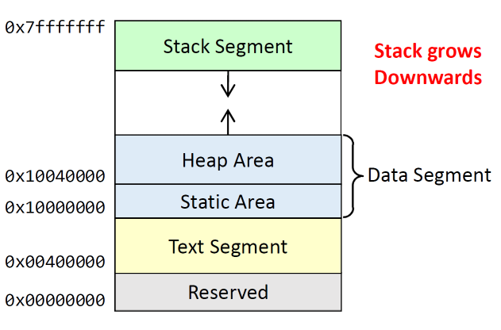
\includegraphics[width=\linewidth]{mips_memory_stack.png}
				\caption{MIPS Memory Organization}
			\end{figure}
		\end{column}
	\end{columns}
\end{frame}

\section{Examples}
\begin{frame}[fragile]
	\frametitle{Recursive Function Example} 
	\begin{columns}[c]
		\begin{column}{0.4\textwidth}
					
			\begin{listing}[H]
			\centering			
			\caption{Recursive factorial function}
			\begin{minted}[frame=single,autogobble,xleftmargin=0.1\textwidth,xrightmargin=0.1\textwidth,framesep=2mm,baselinestretch=1.2,fontsize=\fontsize{7pt}{8pt}\selectfont,obeytabs,tabsize=2]{c}
			int fact(int n){
				if (n < 2)
					return 1;
				else
					return n*fact(n-1);
			}
			\end{minted}
			\end{listing}
			
		\end{column}
		\begin{column}{0.6\textwidth}
			Recursive factorial function in MIPS Assembly
			\minibox[frame,pad=1pt,t]{
					\fontsize{8pt}{9pt}\selectfont fact: \vspace{-0.25cm}\\ 
					\fontsize{8pt}{9pt}\selectfont \hspace{0.5cm}\color{blue}bge \color{red}\$a0\color{black}, 2, else 							 							\hspace{0.28cm}			\color{darkGreen}\# branch if (n $>=$ 2) to else  \vspace{-0.22cm}\\
					\fontsize{8pt}{9pt}\selectfont \hspace{0.5cm}\color{blue}li  \color{red}\$v0\color{black}, 1       							 							\hspace{1.27cm} 		\color{darkGreen}\# \$v0 = 1  \vspace{-0.22cm}\\ 
					\fontsize{8pt}{9pt}\selectfont \hspace{0.5cm}\color{blue}jr  \color{red}\$ra            		   							 							\hspace{1.56cm}			\color{darkGreen}\# return to caller \vspace{-0.22cm}\\ 
					\fontsize{8pt}{9pt}\selectfont else:\vspace{-0.25cm} \\ 
					\fontsize{8pt}{9pt}\selectfont \hspace{0.5cm}\color{blue}addi \color{red}\$sp\color{black}, \color{red}\$sp\color{black}, -8 							\hspace{0.18cm}			\color{darkGreen}\# allocate 8 bytes in the stack\vspace{-0.22cm}\\ 
					\fontsize{8pt}{9pt}\selectfont \hspace{0.5cm}\color{blue}sw   \color{red}\$a0\color{black}, 0(\color{red}\$sp\color{black})  							\hspace{0.45cm}  		\color{darkGreen}\# save the argument n  \vspace{-0.22cm}\\ 
					\fontsize{8pt}{9pt}\selectfont \hspace{0.5cm}\color{blue}sw   \color{red}\$ra\color{black}, 4(\color{red}\$sp\color{black})  							\hspace{0.47cm}  		\color{darkGreen}\# save the return address \vspace{-0.22cm}\\
					\fontsize{8pt}{9pt}\selectfont \hspace{0.5cm}\color{blue}addi \color{red}\$a0\color{black}, \color{red}\$a0\color{black}, -1 							\hspace{0.12cm}			\color{darkGreen}\# argument \$a0 = n-1  \vspace{-0.22cm}\\
					\fontsize{8pt}{9pt}\selectfont \hspace{0.5cm}\color{blue}jal  \color{black}fact          							  		 							\hspace{1.37cm}			\color{darkGreen}\# call fact(n-1) \vspace{-0.22cm}\\
					\fontsize{8pt}{9pt}\selectfont \hspace{0.5cm}\color{blue}lw   \color{red}\$a0\color{black}, 0(\color{red}\$sp\color{black})  							\hspace{0.45cm}  		\color{darkGreen}\# restore \$a0 = n \vspace{-0.22cm}\\
					\fontsize{8pt}{9pt}\selectfont \hspace{0.5cm}\color{blue}lw   \color{red}\$ra\color{black}, 4(\color{red}\$sp\color{black})  							\hspace{0.50cm}  		\color{darkGreen}\# restore return address \vspace{-0.22cm}\\
					\fontsize{8pt}{9pt}\selectfont \hspace{0.5cm}\color{blue}mul  \color{red}\$v0\color{black}, \color{red}\$a0\color{black}, \color{red}\$v0\color{black} 	\hspace{0.02cm} 		\color{darkGreen}\# \$v0 = n * fact(n-1) \vspace{-0.22cm}\\
					\fontsize{8pt}{9pt}\selectfont \hspace{0.5cm}\color{blue}addi \color{red}\$sp\color{black}, \color{red}\$sp\color{black}, 8  							\hspace{0.18cm}  		\color{darkGreen}\# free stack frame \vspace{-0.22cm}\\
					\fontsize{8pt}{9pt}\selectfont \hspace{0.5cm}\color{blue}jr   \color{red}\$ra\color{black}             						 							\hspace{1.58cm}	 		\color{darkGreen}\# return to the caller\\

			}		
		\end{column}
	\end{columns}
\end{frame}

\begin{frame}
	\frametitle{Live Examples}
	
\end{frame}

%------------------------------------------------

\section{Tasks}

\begin{frame}
	\frametitle{Task \#1}
	\begin{columns}[c]
		\begin{column}{0.5\textwidth}
			\justifying
			Write a MIPS assembly program that that implements the read, reverse, and print functions used by f function in Figure 7.6 \& Figure 7.7 in the PDF file. These functions should work with any size n (not only size 10). Then write a main function that calls function f.
			\vspace{0.15cm}
		\end{column}
		\begin{column}{0.5\textwidth}
			\begin{figure}
				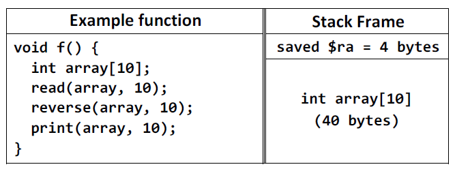
\includegraphics[width=\linewidth]{f_code.png}
				\caption{f function in C}
			\end{figure}
			\vspace{-0.40cm}
			\begin{figure}
				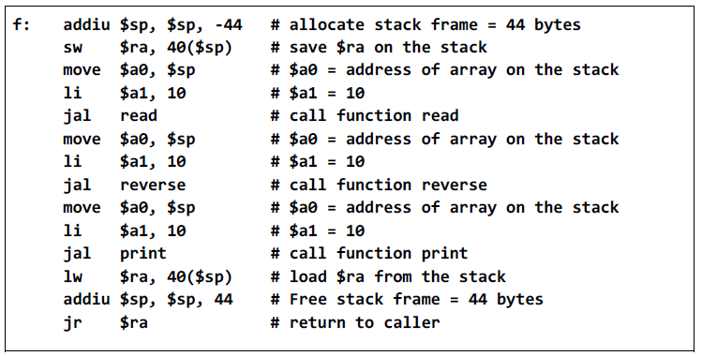
\includegraphics[width=\linewidth]{f_function.png}
				\caption{f function in MIPS Assembly}
			\end{figure}
		\end{column}
	\end{columns}
\end{frame}

\begin{frame}
	\frametitle{Task \#1}
	\centering
	Sample Run 


	\minibox[frame,pad=1pt]{
		\fontsize{6pt}{7pt}\color{black}Enter integer 1: \color{blue}1 \\
		\fontsize{6pt}{7pt}\color{black}Enter integer 2: \color{blue}2 \\
		\fontsize{6pt}{7pt}\color{black}Enter integer 3: \color{blue}3 \\
		\fontsize{6pt}{7pt}\color{black}Enter integer 4: \color{blue}4 \\
		\fontsize{6pt}{7pt}\color{black}Enter integer 5: \color{blue}5 \\
		\fontsize{6pt}{7pt}\color{black}Enter integer 6: \color{blue}6 \\
		\fontsize{6pt}{7pt}\color{black}Enter integer 7: \color{blue}7 \\
		\fontsize{6pt}{7pt}\color{black}Enter integer 8: \color{blue}8 \\
		\fontsize{6pt}{7pt}\color{black}Enter integer 9: \color{blue}9 \\
		\fontsize{6pt}{7pt}\color{black}Enter integer 10: \color{blue}10 \\
		\fontsize{6pt}{7pt}\color{black}Integer reversed = \color{darkGreen}10 9 8 7 6 5 4 3 2 1 \\
	}
\end{frame}

\begin{frame}[fragile]
	\frametitle{Task \#2}
	\begin{columns}[c]
		\begin{column}{0.5\textwidth}
			\justifying
			Write a MIPS assembly program that asks the user for an integer \underline{\textbf{n}} he wishes to compute the Fibonacci number at that index. Calculate \underline{\textbf{fib(n)}} based on the following code. Finally, print out the result.
		\end{column}
		\begin{column}{0.5\textwidth}
		\centering
			\begin{listing}[H]
			\centering			
			\caption{Recursive Fibonacci function}
			\begin{minted}[frame=single,autogobble,xleftmargin=0.1\textwidth,xrightmargin=0.1\textwidth,framesep=2mm,baselinestretch=1.2,fontsize=\footnotesize,obeytabs,tabsize=2]{c}
int fib(int n) {
	if (n <= 1) 
		return n;
	return fib(n-1)+fib(n-2);
}
			\end{minted}
			\end{listing}

			\vspace{0.15cm}
			\centering
			Sample Run 

			\minibox[frame,pad=4pt]{
				\color{black}Enter n: \color{blue}7 \\
				\color{black}fib(n) = \color{darkGreen}13 \\
			}
			
		\end{column}
	\end{columns}
\end{frame}

%----------------------------------------------------------------------------------------

\end{document} 
